\documentclass[10pt,twocolumn,letterpaper]{article}

\usepackage{cvpr}
\usepackage{times}
\usepackage{epsfig}
\usepackage{graphicx}
\usepackage{amsmath}
\usepackage{amssymb}
\usepackage{pdfpages}
\usepackage{gensymb}
\usepackage{xcolor}

%%%%%%%%%
% Example of figure inclusion
%\begin{figure}[t]
%\begin{center}
%\fbox{\rule{0pt}{2in} \rule{0.9\linewidth}{0pt}}
%   %\includegraphics[width=0.8\linewidth]{egfigure.eps}
%\end{center}
%   \caption{Example of caption.  It is set in Roman so that mathematics
%   (always set in Roman: $B \sin A = A \sin B$) may be included without an
%   ugly clash.}
%\label{fig:long}
%\label{fig:onecol}
%\end{figure}

%%%%%%%%%
% Example table
%\noindent
%Compare the following:\\
%\begin{tabular}{ll}
% \verb'$conf_a$' &  $conf_a$ \\
% \verb'$\mathit{conf}_a$' & $\mathit{conf}_a$
%\end{tabular}\\
%
%
%
%\begin{table}
%\begin{center}
%\begin{tabular}{|l|c|}
%\hline
%Method & Frobnability \\
%\hline\hline
%Theirs & Frumpy \\
%Yours & Frobbly \\
%Ours & Makes one's heart Frob\\
%\hline
%\end{tabular}
%\end{center}
%\caption{Results.   Ours is better.}
%\end{table}

%%%%%%%%%
% another example figure
%\begin{figure*}
%\begin{center}
%\fbox{\rule{0pt}{2in} \rule{.9\linewidth}{0pt}}
%\end{center}
%   \caption{Example of a short caption, which should be centered.}
%\label{fig:short}
%\end{figure*}
%
%
%%%%%%%%%
% example citation
%   Frobnication has been trendy lately.
%   It was introduced by Alpher~\cite{Alpher02}, and subsequently developed by
%   Alpher and Fotheringham-Smythe~\cite{Alpher03}, and Alpher \etal~\cite{Alpher04}.''

    %Figure and table captions should be 9-point Roman type as in
    %Figures~\ref{fig:onecol} and~\ref{fig:short}.  Short captions should be centred.
% Include other packages here, before hyperref.

% If you comment hyperref and then uncomment it, you should delete
% egpaper.aux before re-running latex.  (Or just hit 'q' on the first latex
% run, let it finish, and you should be clear).
%
% When placing figures in \LaTeX, it's almost always best to use
% \verb+\includegraphics+, and to specify the  figure width as a multiple of
% the line width as in the example below
% {\small\begin{verbatim}
%    \usepackage[dvips]{graphicx} ...
%       \includegraphics[width=0.8\linewidth]
%           {myfile.eps}
%   \end{verbatim}
% }
%
\usepackage[breaklinks=true,bookmarks=false]{hyperref}

\cvprfinalcopy % *** Uncomment this line for the final submission

\def\cvprPaperID{****} % *** Enter the CVPR Paper ID here
\def\httilde{\mbox{\tt\raisebox{-.5ex}{\symbol{126}}}}

% Pages are numbered in submission mode, and unnumbered in camera-ready
%\ifcvprfinal\pagestyle{empty}\fi
\setcounter{page}{1}
\begin{document}

%%%%%%%%% TITLE
\title{Predicting the Eye Fixations with Prior Knowledge: \\A Bayesian Learning Architecture}

\author{Lauren Arnett and Chengzhi Mao\\
Columbia University in the City of New York\\
    {\tt\small \{lba2138,cm3797\}@columia.edu}
    \\\href{https://github.com/laurenarnett/eye-movements}{\small\color{blue} Link to GitHub
    Repository}
}

\maketitle

%%%%%%%%% ABSTRACT
\begin{abstract} 
    
    Applications of tracking eye fixation location span from neuroscience and
    the study of human vision to advertising and human computer interaction. By
    creating a model to generate a prediction of where the eye may be most
    attracted to, industries can circumvent the expense of running studies on
    eye-tracking with actual human subjects. We look to improve upon existing
    models of saliency by using Bayesian methods with deep learning techniques.

\end{abstract}

%%%%%%%%% BODY TEXT
\section{Introduction} It is estimated that 80\% of all external sensory input
processed by the human brain is processed by the visual pathway~\cite{Jerath}.
As such, optimizing image layout for processing by the human brain allows for
better information retrieval and retention across the image. Studying how
humans’ eyes move across images is thus relevant for fields from neuroscience
to advertising and  art. Being able to predict where humans are most likely to
look provides a guideline as to whether the image has an effective layout, what
humans are attracted to in viewing art, or how an image should be cropped to
feature the subject. Using an existing dataset of eye movements, we build
a predictive model to generate the most likely fixation locations on a new
image.

Our main contribution in this paper is combining Bayesian methods with deep
learning to perform the eye-fixation prediction task. We also explore a dataset
of fixation locations that has not yet been used for the fixation prediction
task. Additionally, we introduce a method to use an auxiliary dataset to learn
image priors based on the area of the image that encodes the most semantic
meaning. 

%-------------------------------------------------------------------------
\section{Related Work} 

Traditionally, studies on eye movements have been carried out such that
viewers look at images on a monitor while an eye tracker records the
eye-fixations that stay within a threshold angle of movement. This procedure is
very costly, and necessitated formulating a method to predict where users will
look. Thus, models of saliency---the likelihood of a location to attract the
visual attention of a human---developed that are modeled mathematically using
biologically plausible linear filters. For example, linear combinations of
filters for low-level features such as color, intensity, and orientation
filters can be used to compute a total saliency map for an image,
providing a bottom-up understanding of the image~\cite{Itti}.

These models do not account for particular tasks that the viewer may have in
looking at the image, and often do not align with the ground truth fixation
locations. Judd \etal~\cite{Judd} propose using deep learning for this task
rather than deriving mathematical models and show that training from a large
database of eye-tracking data outperforms existing models. K\"ummerer
\etal~\cite{Kummerer} also employ deep learning for predicting fixation
locations, using the AlexNet architecture in \textit{DeepGaze I} and building
upon the VGG-19 network in \textit{DeepGaze II}.

Developing a dataset for use by saliency models is also a field of exploration.
Judd \etal~\cite{Judd} create a dataset of 1003 images with the fixation
locations from 15 viewers each and make it publicly available. Jiang
\etal~\cite{Jiang} relies on an assumption of eye-mouse coordination---they
simulate recording eye-tracking data by instead recording mouse-tracking data
using Amazon Mechanical Turk. This provides a less expensive and
training-intensive method of developing a simulated saliency map. Finally, the
MIT300 dataset \cite{mitbench} looks to provide a performance benchmark for new predictive
models for saliency, with performance statistics for over 80 models at the time
of writing. 


\section{Dataset}
We make use of two datasets: ImageNet \cite{imagenet} for the train set for our prior and an
eye-fixation dataset for our classifier. 

\subsection{Use of ImageNet for Training a Prior}
We use the complete training set with the original image and the label
information of ImageNet for training our prior. We select the best prior model
based on the performance on the validation set. 

\subsection{Source for Eye-Tracking Data}
We use an open-source dataset developed at Osnabr\"uck University and the
University Medical Center in Hamburg-Eppendorf \cite{Wilming01, Wilming02}. This dataset comprises images
of many categories, including urban and rural settings, fractals, faces, and
websites. For our purposes, we use the images of urban and rural settings,
which have been taken from the LabelMe dataset \cite{labelme}. Each image in
this category is shown to the viewer for eight seconds, and this category has
the x- and y-coordinates of 70,026 fixation locations for seven observers over
600 images. Figure ~\ref{fig:dataset} shows examples of fixation locations
across the image. We use a 500/100 train/test split.
\begin{figure}
    \begin{center}
        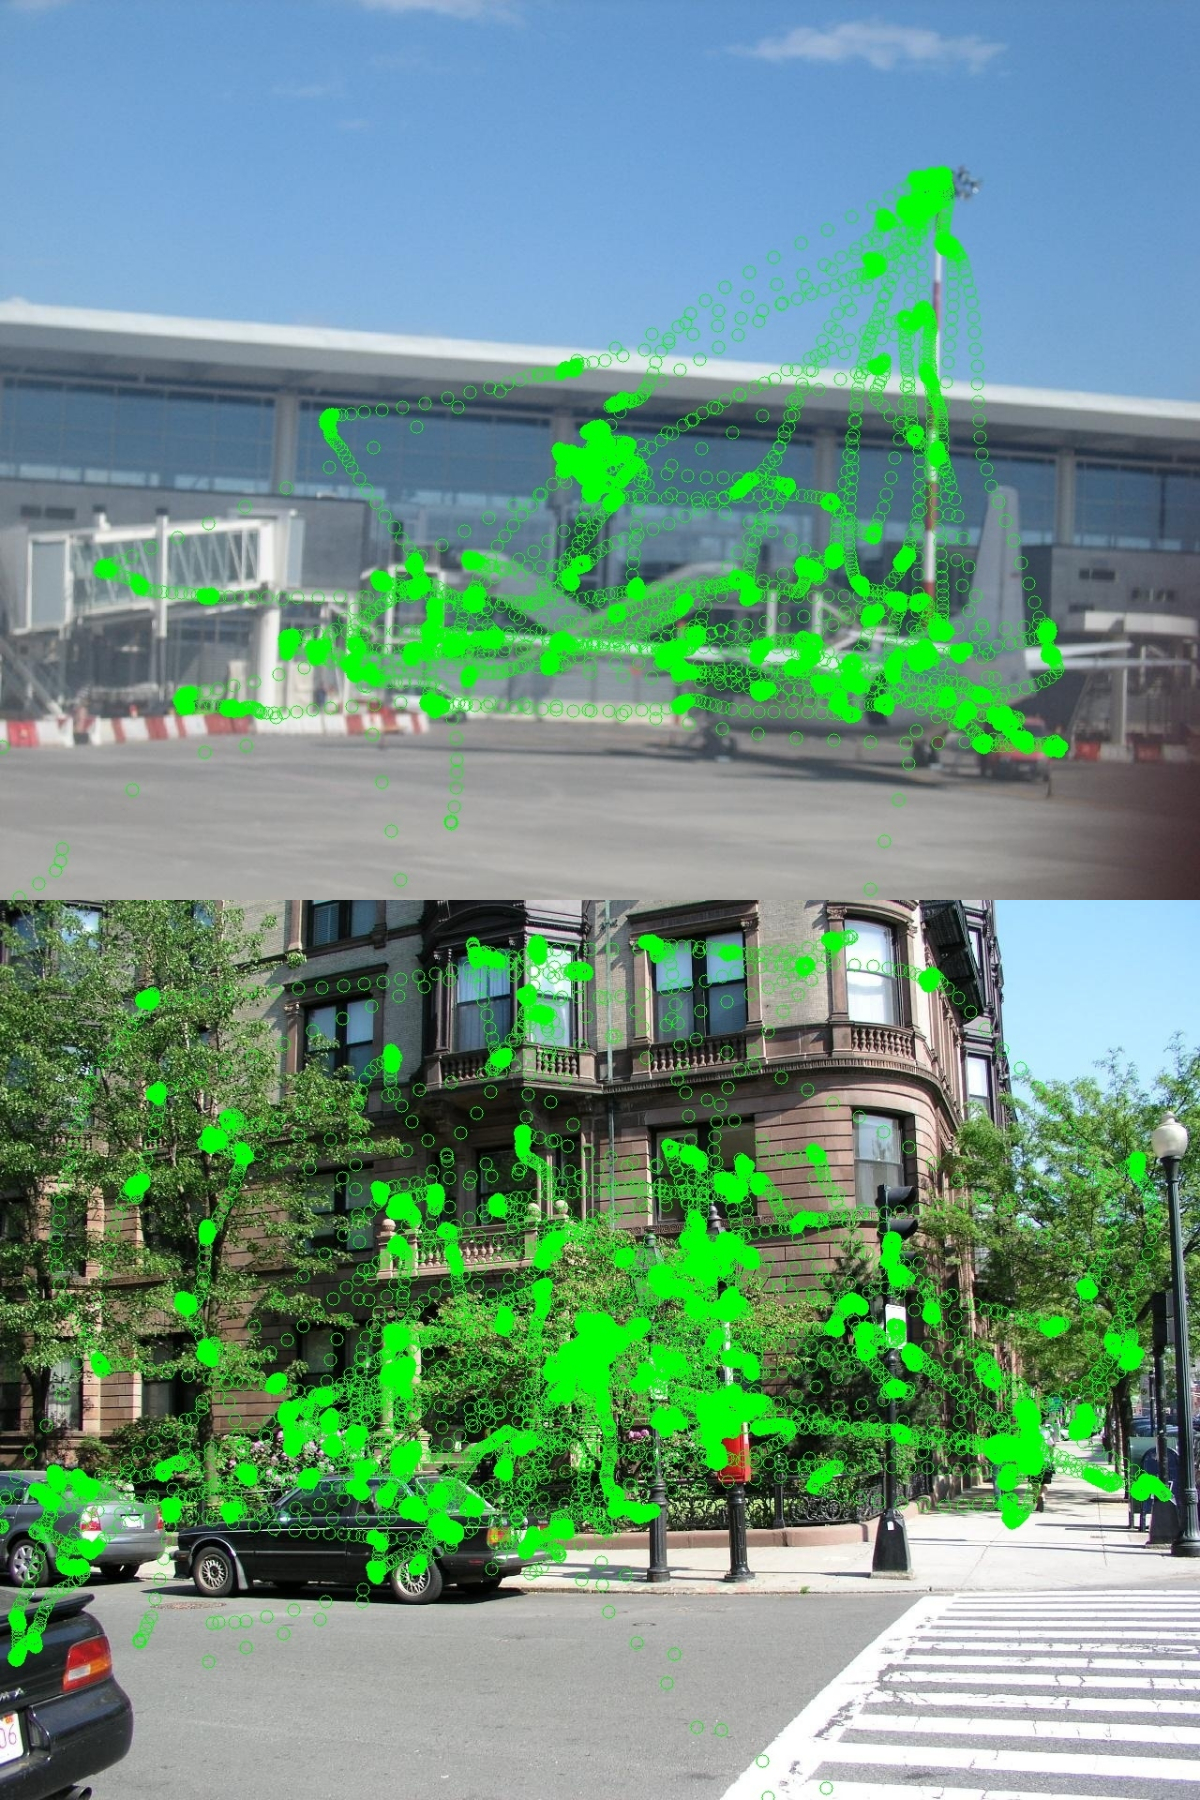
\includegraphics[width=0.5\columnwidth]{figures/movements.jpg}
    \end{center}
    \caption{Eye-tracking locations on sample images from dataset.}
    \label{fig:dataset}
\end{figure}

\subsection{Preprocessing} We preprocess the fixation data by adding weight to
those pixels in the image that have fixations to produce ground truth labels.
We apply a Gaussian blur to also add weight to neighboring pixels to account
for the $0.5\degree$ angle of error due to the eye-tracking machine.
Figure~\ref{fig:preprocess} shows the fixation locations and corresponding
ground truth labels.

\begin{figure}
	\begin{center}
		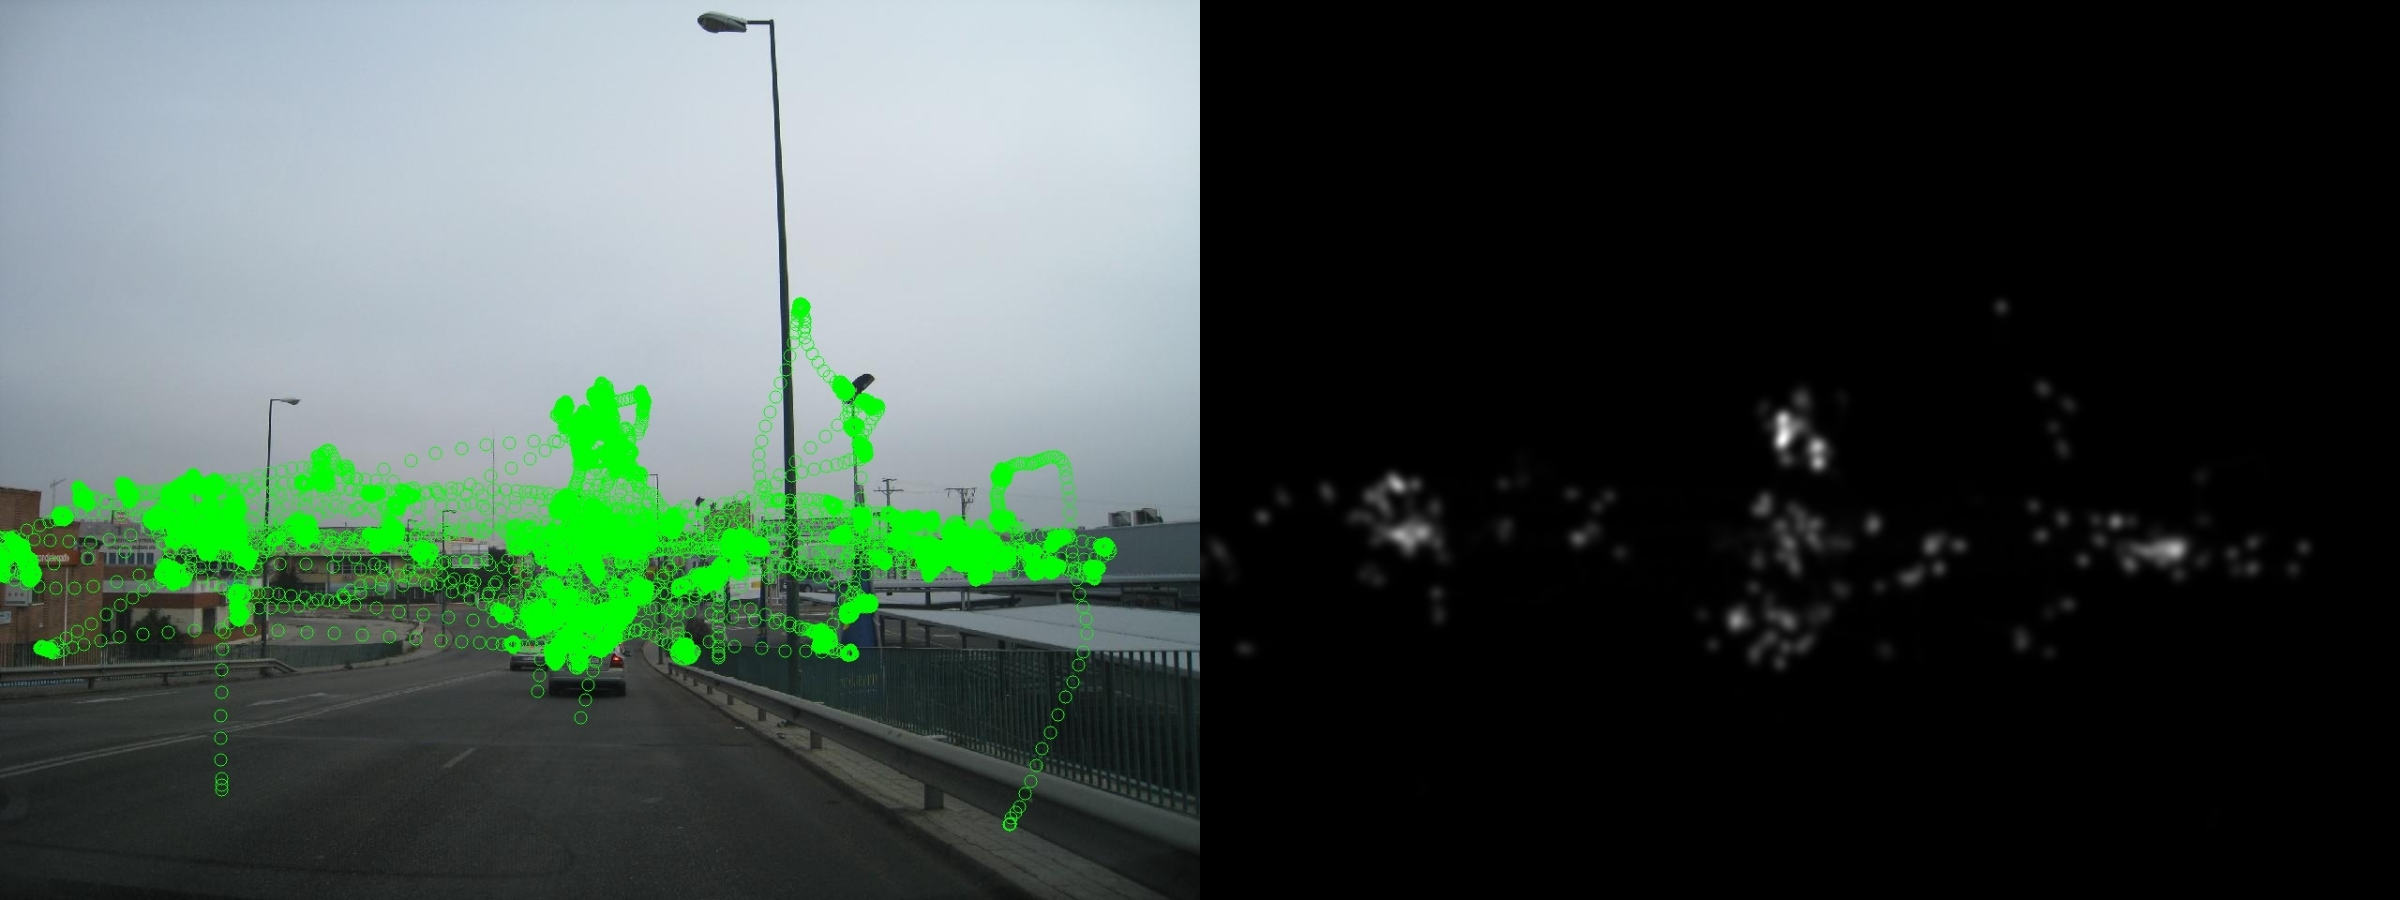
\includegraphics[width=\columnwidth]{figures/preprocess.png}
	\end{center}
	\caption{Preprocessing of the fixation locations.}
	\label{fig:preprocess}
\end{figure}


\section{Learning a Model}
\subsection{Baseline Model Setting}

We conduct a binary classification task for each output pixel in our baseline
eye fixation model. We propose a U-Net architecture, using a fixed pretrained
VGG model. We take the features of layer numbers 3, 8, 15, and 22 in the VGG
model and feed them into our fixation prediction network. We first learn
a upsampling of the high-level, low-resolution features of VGG, and then
concatenate it with the low-level, high-resolution features to produce a final
prediction.

 \begin{figure}
	\begin{center}
		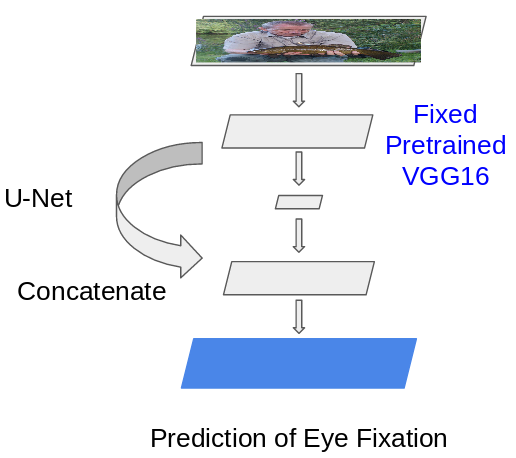
\includegraphics[width=\columnwidth]{figures/architecture_bl.png}
	\end{center}
	\caption{U-Net Architecture for our baseline model.}
	\label{fig:unet}
\end{figure}

\subsection{Overcoming the Checkerboard Artifacts of Upsampling} Building the
upsampling using the deconvolution operation introduces checkerboard artifacts,
as shown in Figure \ref{fig:checker}. This is partly due to the overlap of the
deconvolution, according to Odena \etal \cite{checkerboard}. We overcome this
by first sequencing a nearest-neighbor interpolation along with a normal
convolution operation.


 \begin{figure}
	\begin{center}
		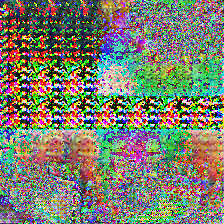
\includegraphics[width=0.4\columnwidth]{figures/checker.png}
	\end{center}
	\caption{Example of checkerboard artifacts.}
	\label{fig:checker}
\end{figure}
\subsection{Learning Prior from the ImageNet}

 Due to the high cost of collecting eye movement data, which requires subjects
 to sit in front of the computer with an expensive eye-tracking machine, the
 number of samples that could be acquired in a training set may be limited. We
 make an attempt to address these challenges by utilizing some prior knowledge
 of eye fixation from an auxiliary dataset.
 
 \begin{figure}
 	\begin{center}
 		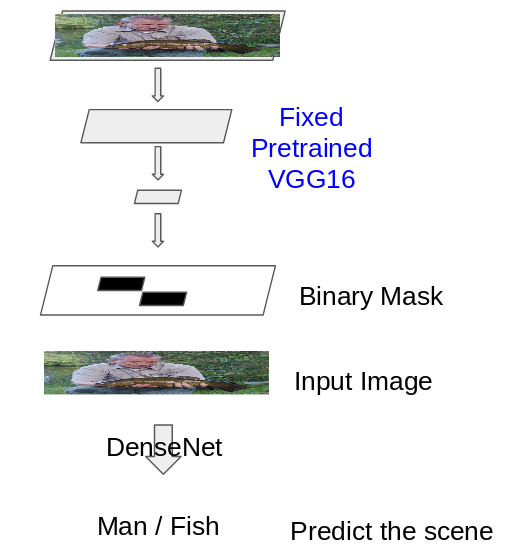
\includegraphics[width=\columnwidth]{figures/Prior.png}
 		
 	\end{center}
 	\caption{Architecture for learning the prior}
 	\label{fig:prior}
 \end{figure}
 
 We interpret eye fixation points as the places which encode the most semantic
 information for the image. With this prior, we construct a model which
 predicts a binary mask with 0 and 1 to select the appropriate locations of the
 image. Applying this binary mask to the image, we then use a neural network to
 predict the semantic information of the masked image. 
 
 The elements with value 1 in the predicted binary mask mimic saliency map,
 where the selection of these points should maximize the semantic information
 in the resulting image after training.
 
 We denote the semantic label of a given image $x_i$ as $y_i$, the predicted mask
 as $M$, and the loss function as $L$,

 $$M_i = F_1(x_i, k)$$
 $$L(X, Y) = \sum_{x_i \in X}{logP(y_i | F_2(M_i * x_i))}$$
 
 \noindent where * denotes element-wise multiplication and $k$ denotes the
 number of elements we use in the binary mask. Here, $F_1$ denotes the
 mask-prediction network, and $F_2$ denotes the pretrained classification
 network. 
 
 After training, the $M_i$ can be interpreted as a learned prior knowledge,
 which is fixed during the Bayesian learning procedure.
 
 \subsection{Incorporating Prior Improves Prediction}
 
 The main contribution of our work is a Bayesian inference procedure that
 builds upon a prior knowledge learned with our auxiliary dataset. We denote
 the eye-fixation ground truth as $t$, 
 
 $$L = logP(M, t|x) = log(P(M|x)) + log(t|M, x)$$
 
 The prior $M$ gives a good estimation of the eye fixation in advance, which
 enhances the optimization achieved by this loss function.
 
 
 
\subsection{Training}
We train our baseline model using SGD, with a learning rate of $1$e$-5$ and
weight decay of $1$e$-6$. We train 50 epoch before we stop.

We use ImageNet data for our prior training, where the mask prediction network
is based on a pretrained VGG--16 network, and the network to predict semantic
meaning from the masked image is a DenseNet, which we believe to have more
accurate gradient information. We train this mask prediction network using SGD
with a learning rate of 1e$-5$.

\subsection{Evaluating the Prior} We visualize our binary mask prediction using
both ImageNet and our fixation dataset. In Figure \ref{fig:birdmask}, we show
the output of applying the mask to an ImageNet sample. This output is in line
with expectations of eye-fixations on the bird. We then extrapolate our learned
prior model for usage with our eye-fixation dataset, as seen in Figure
\ref{fig:street}.  Through visualizing the application of the mask across
images in our eye-fixation dataset, we see that the prior, after training on
ImageNet, is able to generalize to the new dataset.

\begin{figure}
	\begin{center}
		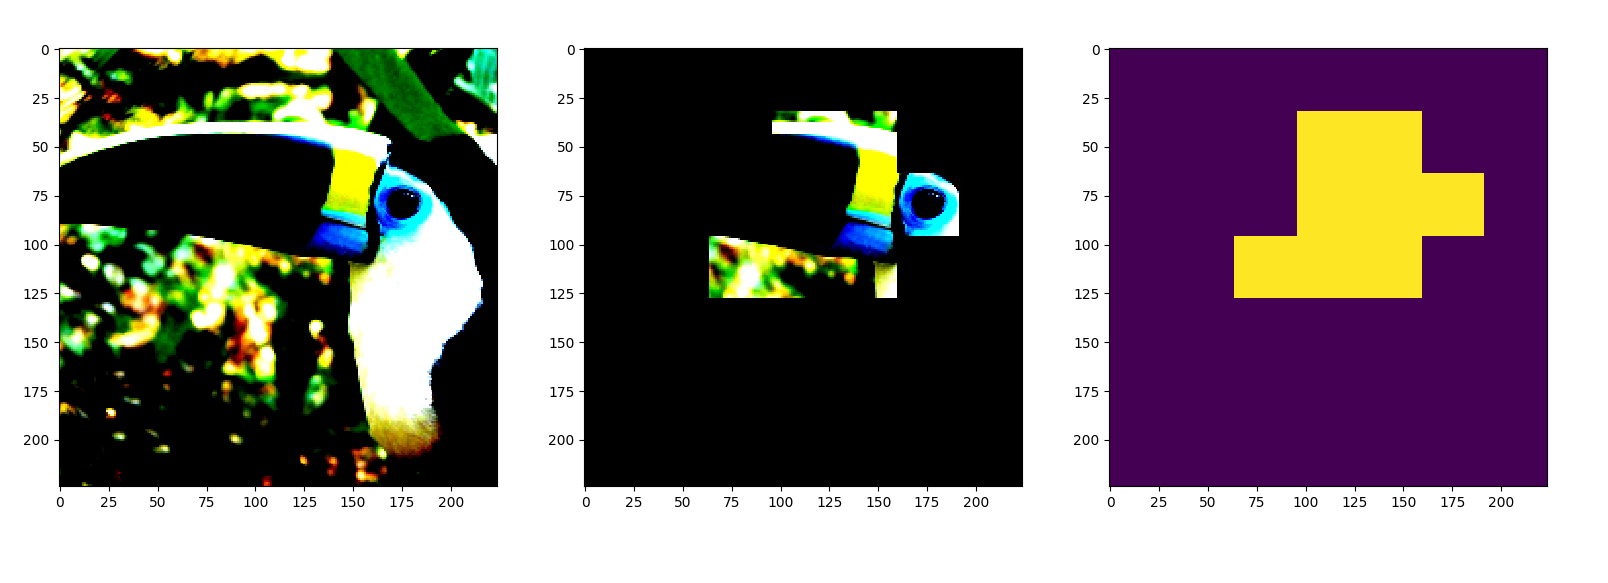
\includegraphics[width=\columnwidth]{figures/bird_mask_predict.png}
		
	\end{center}
	\caption{Example of mask learned on ImageNet}
	\label{fig:birdmask}
\end{figure}

\begin{figure}
	\begin{center}
		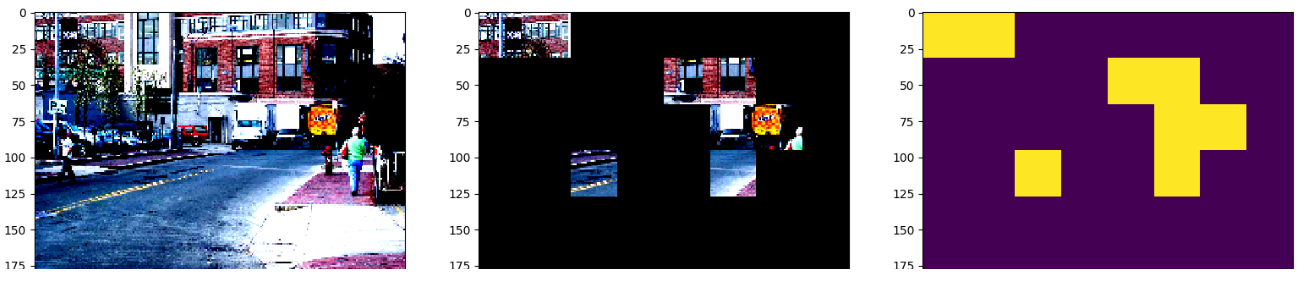
\includegraphics[width=\columnwidth]{figures/road.png}		
	\end{center}
	\caption{Example of extrapolating the prior learned on ImageNet to the eye fixation dataset}
	\label{fig:street}
\end{figure}

\subsection{Evaluation Metric}

In accordance with Judd \etal~\cite{Judd}, we use the true positive rate
$\frac{TP}{TP + FN}$ as the evaluation metric, where $TP$ is number of true positives, and $FN$ is the
number of false negatives. This is evaluated using the probability prediction
output of how salient each pixel is. We threshold this saliency map at the top
$k$ percent probability, where $k=1, 3, 5, 10, 15, 20, 25$ and 30 percent of
the image saliency map. 

\subsection{Performance}
Figure \ref{fig:tpr} shows our model's performance. We draw the ROC curve for the true
positive rate. We can see that the Bayesian model outperforms the baseline
model by a large margin. Specifically, at the 10\% threshold for the saliency map, the
performance of the baseline model achieves 94.1\% performance of the Bayesian
model, and at the 30\% threshold, the baseline model achieves 97\% performance
of the Bayesian model.

\begin{figure}
\begin{center}
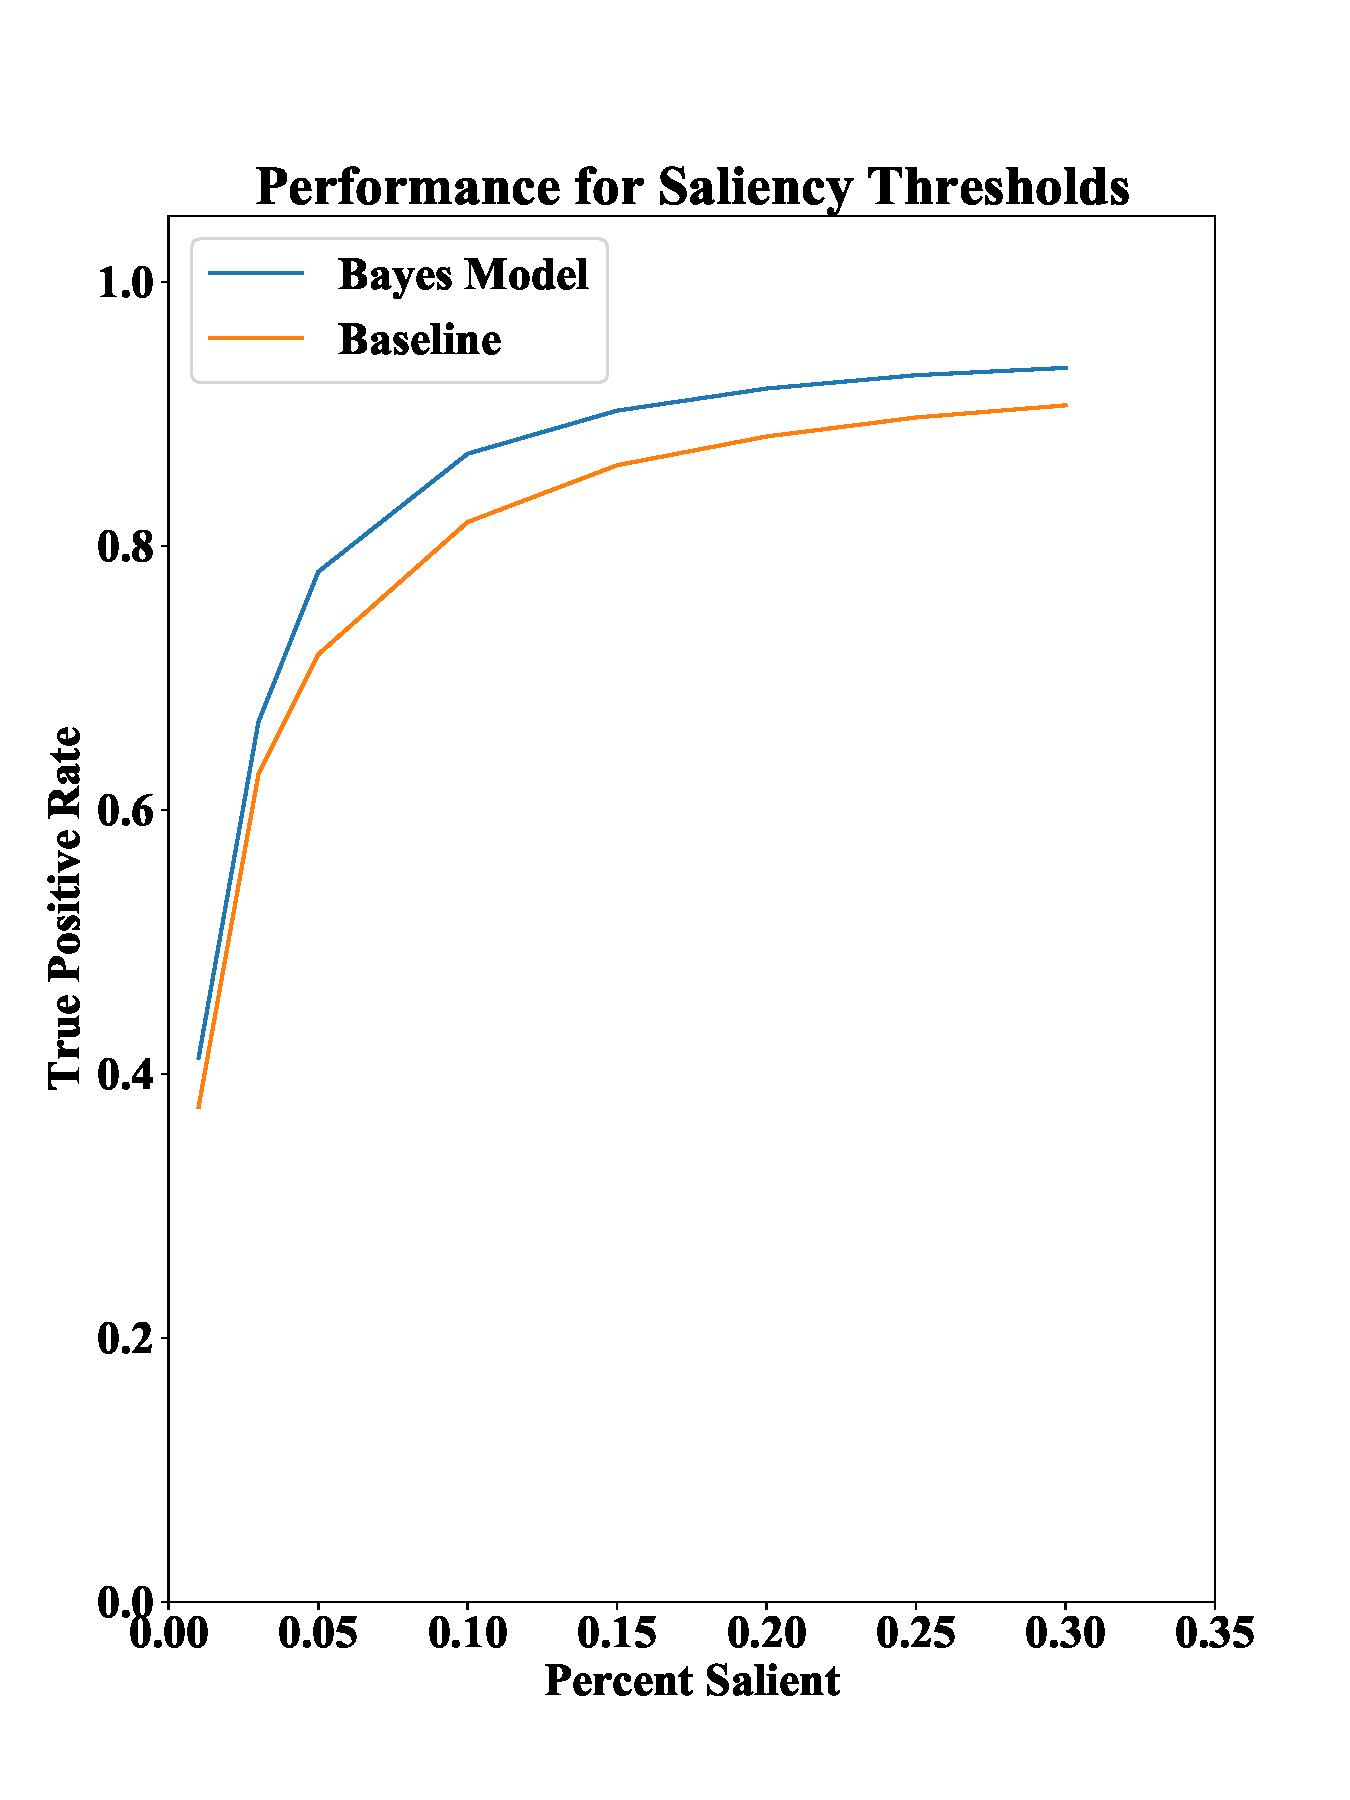
\includegraphics[width=\columnwidth]{figures/tpr.pdf}

\end{center}
   \caption{Example of a short caption, which should be centered.}
\label{fig:tpr}
\end{figure}

\section{Conclusion} Our study looks at using new methods and a new dataset for
the task of predicting eye-fixation locations. We use a subset of a large
dataset of fixation locations to account for the difficulty of obtaining such
data.  By combining a neural network classification model with a learned image
prior, we achieve a higher performance than that of our classifier alone. 

%------------------------------------------------------------------------
{\small
\bibliographystyle{ieee}
\bibliography{egbib}
}

\end{document}
